
\section{Finding the most Optimized Arbitrage Bet}

We have learnt how to find arbitrage bets in the previous section. Now we will learn how to find the most optimized arbitrage bet. This is done by finding the most optimized arbitrage bet in the following way:

We look at $n$ amount of bookmakers $B_{}$. We formulate a matrix of $O_{n}$ odds for the same match $M_{n}$\\

I wrote the odds in a form $O{oddtype,matrixentrynumber}$ in the matrix\\

\begin{equation}
    M_{n} = \begin{bmatrix}
        B_{1} & B_{2} & B_{3} & \dots & B_{n} \\
        O_{1,1} & O_{2,3} & O_{3,5} & \dots & O_{4,7} \\
        O_{1,2} & O_{2,4} & O_{3,6} & \dots & O_{4,8} \\
        \vdots & \vdots & \vdots & \ddots & \vdots \\
        O_{1,k} & O_{2,k+1} & O_{3,k+2} & \dots & O_{4,k+3} \\
    \end{bmatrix}
\end{equation}

We then find the most optimized arbitrage bet by finding the maximum value for each row in the matrix $M_{n}$

Resulting in a matrix of $O_{n}$ odds for the same match $M_{n}$

\begin{equation}
    Opt_{M_{n}} = \begin{bmatrix}
        B_{x} & B_{y} & B_{z} & \dots & B_{p} \\
        O_{1,maxentry} & O_{2,maxentry} & O_{3,maxentry} & \dots & O_{n,maxentry} \\
    \end{bmatrix}
\end{equation}

Where $B_{var}$ is the bookmaker with the highest odds for the match $M_{n}$

In theory the more bookmakers we have the more optimized our arbitrage bet will be. The more optimized bet results in yielding a higher profit for the arbitrage bet.\\

But always remember for it to be an arbitrage bet the $A_{n}$ must be less than $1$.

\newpage
\section{Python Class to Compute Arbitrage Bets}

Using the Python Class we can compute arbitrage bets. The Python Class is called Arbitrage. \\
I wrote this class based on the mathmatical logic of arbitrage betting as discussed in the previous sections.\\

The Arbitrage class is defined as follows:

\begin{python}
class Arbitrage:
	def __init__(self,odds,investment):self.odds=odds;self.investment=investment
	def is_arbitrage(self):
		arbitrageP=0
		for odd in self.odds:arbitrageP+=1/odd
		if arbitrageP<1:return True
		else:return False
	def calculate_arbitrage_percentage(self):
		arbitrageP=0
		for odd in self.odds:arbitrageP+=1/odd
		return arbitrageP
	def calculate_arbitrage_roi(self):return self.calculate_arbitrage_stats()['returnOnInvestment']
	def calculate_arbitrage_stats(self):
		arbitrageP=self.calculate_arbitrage_percentage();bArbitrage=self.is_arbitrage();actualProfit=self.investment/arbitrageP-self.investment;IndividualBets=[];returnOnInvestment=actualProfit/self.investment*100;returnOnInvestment=str(returnOnInvestment)+'%';Payouts=[]
		for odd in odds:IndividualBets.append(self.investment*(1/odd/arbitrageP));Payouts.append(self.investment*(1/odd/arbitrageP)*odd)
		return{'arbitrageP':arbitrageP,'bArbitrage':bArbitrage,'actualProfit':actualProfit,'IndividualBets':IndividualBets,'returnOnInvestment':returnOnInvestment,'Payouts':Payouts}
\end{python}

Let us do an example of how to use the Arbitrage class.\\

Assumption: We have computed the best odds for a match from different bookmakers.\\

We have resulted in a matrix of odds for the same match.\\

\begin{equation}
    M_{1} = 
    \begin{bmatrix}
        B_{1} & B_{2} & B_{3} \\
        O_{1} = 2.6 & O_{2} = 7.8 & O_{3} = 5 \\ 
    \end{bmatrix}    
\end{equation}

Let our investment $I$ be $R100$

\begin{python}
odds=[2.6,7.8,5]
investment=100
objArbitrage = Arbitrage(odds, investments)
print(objArbitrage.calculate_arbitrage_stats())
\end{python}

The output of the above code is as follows: \\

\begin{python}
{'arbitrageP': 0.7128205128205127, 'bArbitrage': True, 'actualProfit': 40.28776978417267, 'IndividualBets': [53.956834532374096, 17.985611510791372, 28.057553956834536], 'returnOnInvestment': '40.28776978417267%', 'Payouts': [140.28776978417267, 140.2877697841727, 140.28776978417267]}
\end{python}

\subsubsection{Opportunities from this}

% render image from images/ folder
\begin{wrapfigure}{r}{0.28\textwidth}
    \centering
    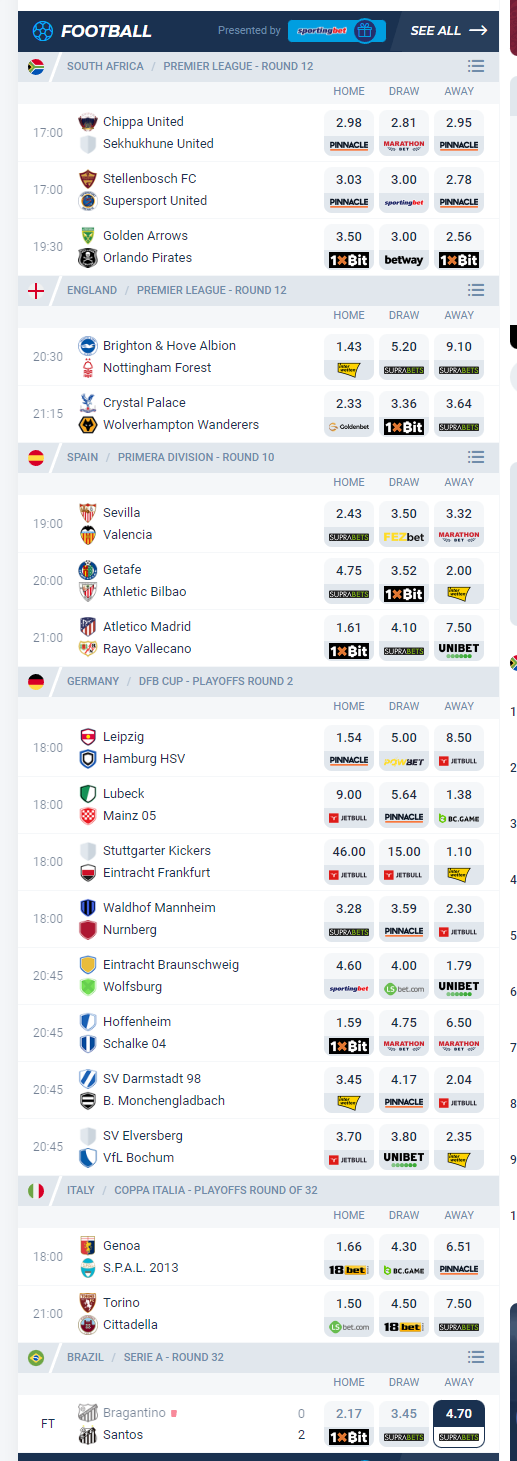
\includegraphics[scale=0.55]{images/oddspedia.png}
    \caption{Oddspedia}
    \label{fig:oddspedia}
\end{wrapfigure}

The above code can be used to compute arbitrage bets.\\

We can use that code to compute arbitrage bets to compute the most optimized arbitrage bet.\\

If we have a matrix of different odds for the same match from different bookmakers. We can compute the most optimized arbitrage bet by finding the maximum value for each row in the matrix $M_{n}$ \\

\begin{math}
    Opt_{n} = \begin{bmatrix}
        B_{x} & B_{y} & B_{z} & \dots & B_{p} \\
        O_{1,maxentry} & O_{2,maxentry} & O_{3,maxentry} & \dots & O_{n,maxentry} \\
    \end{bmatrix}
\end{math} \\

We can introduce Data Science methodologies scrape data from different bookmakers and compute the most optimized arbitrage bet.\\
I wont be showing how to do that in this paper it is up to you to figure that out.\\

There is already websites that do this for you.\\

Example of a website that does this for you: \\ https://oddspedia.com/odds \\

There is also an web application i have developed that does this for you.\\
\\ https://odds.adgstudios.co.za/ \\

It is powered by the Oddspedia API.\\

% center image
\begin{figure}[h]
    \centering
    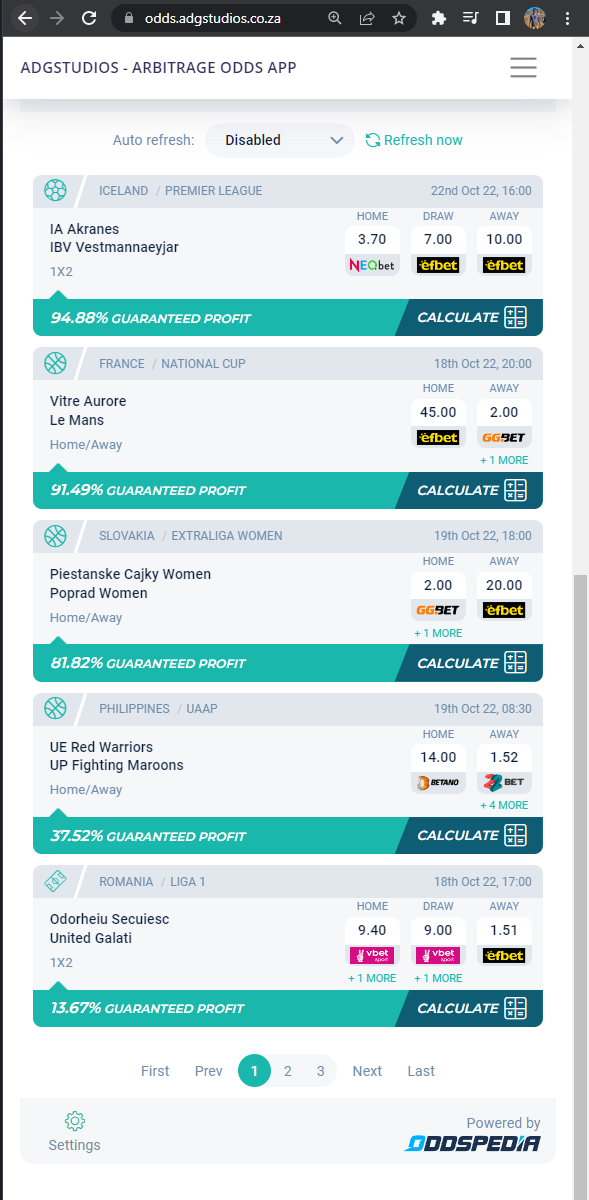
\includegraphics[scale=0.55]{images/arbitrageapp.png}
    \caption{https://odds.adgstudios.co.za/}
    \label{fig:odds}
\end{figure}

\textbf{Limitations of this method:} \\
The websites are not always up to date.\\
Odds change all the time.\\
There are some bookmakers that are not on the websites.\\
Some bookmakers change the odds live during the match.\\
You will have to manually check the odds on the bookmakers website before placing the bet.\\
You will have to have many bookmakers accounts to place the arbitrage bet.\\
Money withdrawal from bookmakers can take a long time.\\





